\section{Introduction} \label{Introduction}

A study revealed that over 24,000 GB of data is uploaded to the internet every second, from which approximately 80\% consists of video data \citep{CiscoInternetStudy}.
Consequently, a vast amount of visual data is generated each second, highlighting the significance of algorithms that are capable of comprehending visual information.

Algorithms that can interpret visual data have various applications, including autonomous vehicles \citep{selfdrivingcars_cnn} that rely on cameras to perceive the environment, analyze it, and make informed decisions based on the gathered data. Additionally, these algorithms are instrumental in fields such as skin cancer detection \citep{skin_cancer_detection_cnn}, crop disease detection \citep{crop_disease_detection} and more. Therefore, the development of algorithms that possess the ability to understand visual data is important.

In computer systems, an image is represented as a matrix, where the size of the matrix corresponds to the dimensions of the image.
This matrix representation poses several challenges for algorithms aiming to understand images, including viewpoint variations, illumination changes, occlusions, background clutter, and more.
For instance, when viewing an image from different perspectives or under different lighting conditions, the semantic meaning of the image remains the same, but the values within the matrix can change drastically.

This brings us to the fundamental question: How can we develop algorithms that can effectively understand images despite the inherent variability in their representations?
One idea is instead of using rigid rules and handcrafted features, we let the computer learn the semantic meaning of images.

\section{Convolutional Neural Network} \label{CNN}

\subsection{Introduction}

Neural Network can serve as universal function approximator \citep{HORNIK1989359}.
This property makes them a suitable candidate for training algorithms that can semantically understand images.
However, as highlighted in \citep{CNNLeCunDocumentRecog}, conventional neural networks are not optimally designed for learning visual data due to the following reasons:
\begin{itemize}
    \item A fully connected Neural Network would take too many parameters, thus being computationally expensive to train.
    \item A fully connected Neural Network has no built-in invariance to image transformations like already named in subsection \ref{Introduction}.
    \item Fully connected Neural Networks(FCNN) ignore how the input is ordered. We could randomly map (fixed) input pixels to the first layer without affecting the training.
\end{itemize}
A more effective approach is to utilize specialized architectures known as convolutional neural networks (CNNs), like introduced in \citep{rumelhart1985learning}, \citep{CNNLeCunHandwrittenDigits}, \citep{CNNLeCunDocumentRecog} and \citep{NIPS2012_c399862d}. CNNs address the limitations faced by traditional neural networks and provide improved performance in handling visual data.

CNNs can learn to semantically understand images, instead of relying on handcrafted features or explicit rules.
CNNs do that by learning a hierarchical representation from the raw pixel data, as seen in figure \ref{fig:cnn_features}.

\begin{figure}[h]
    \centering
    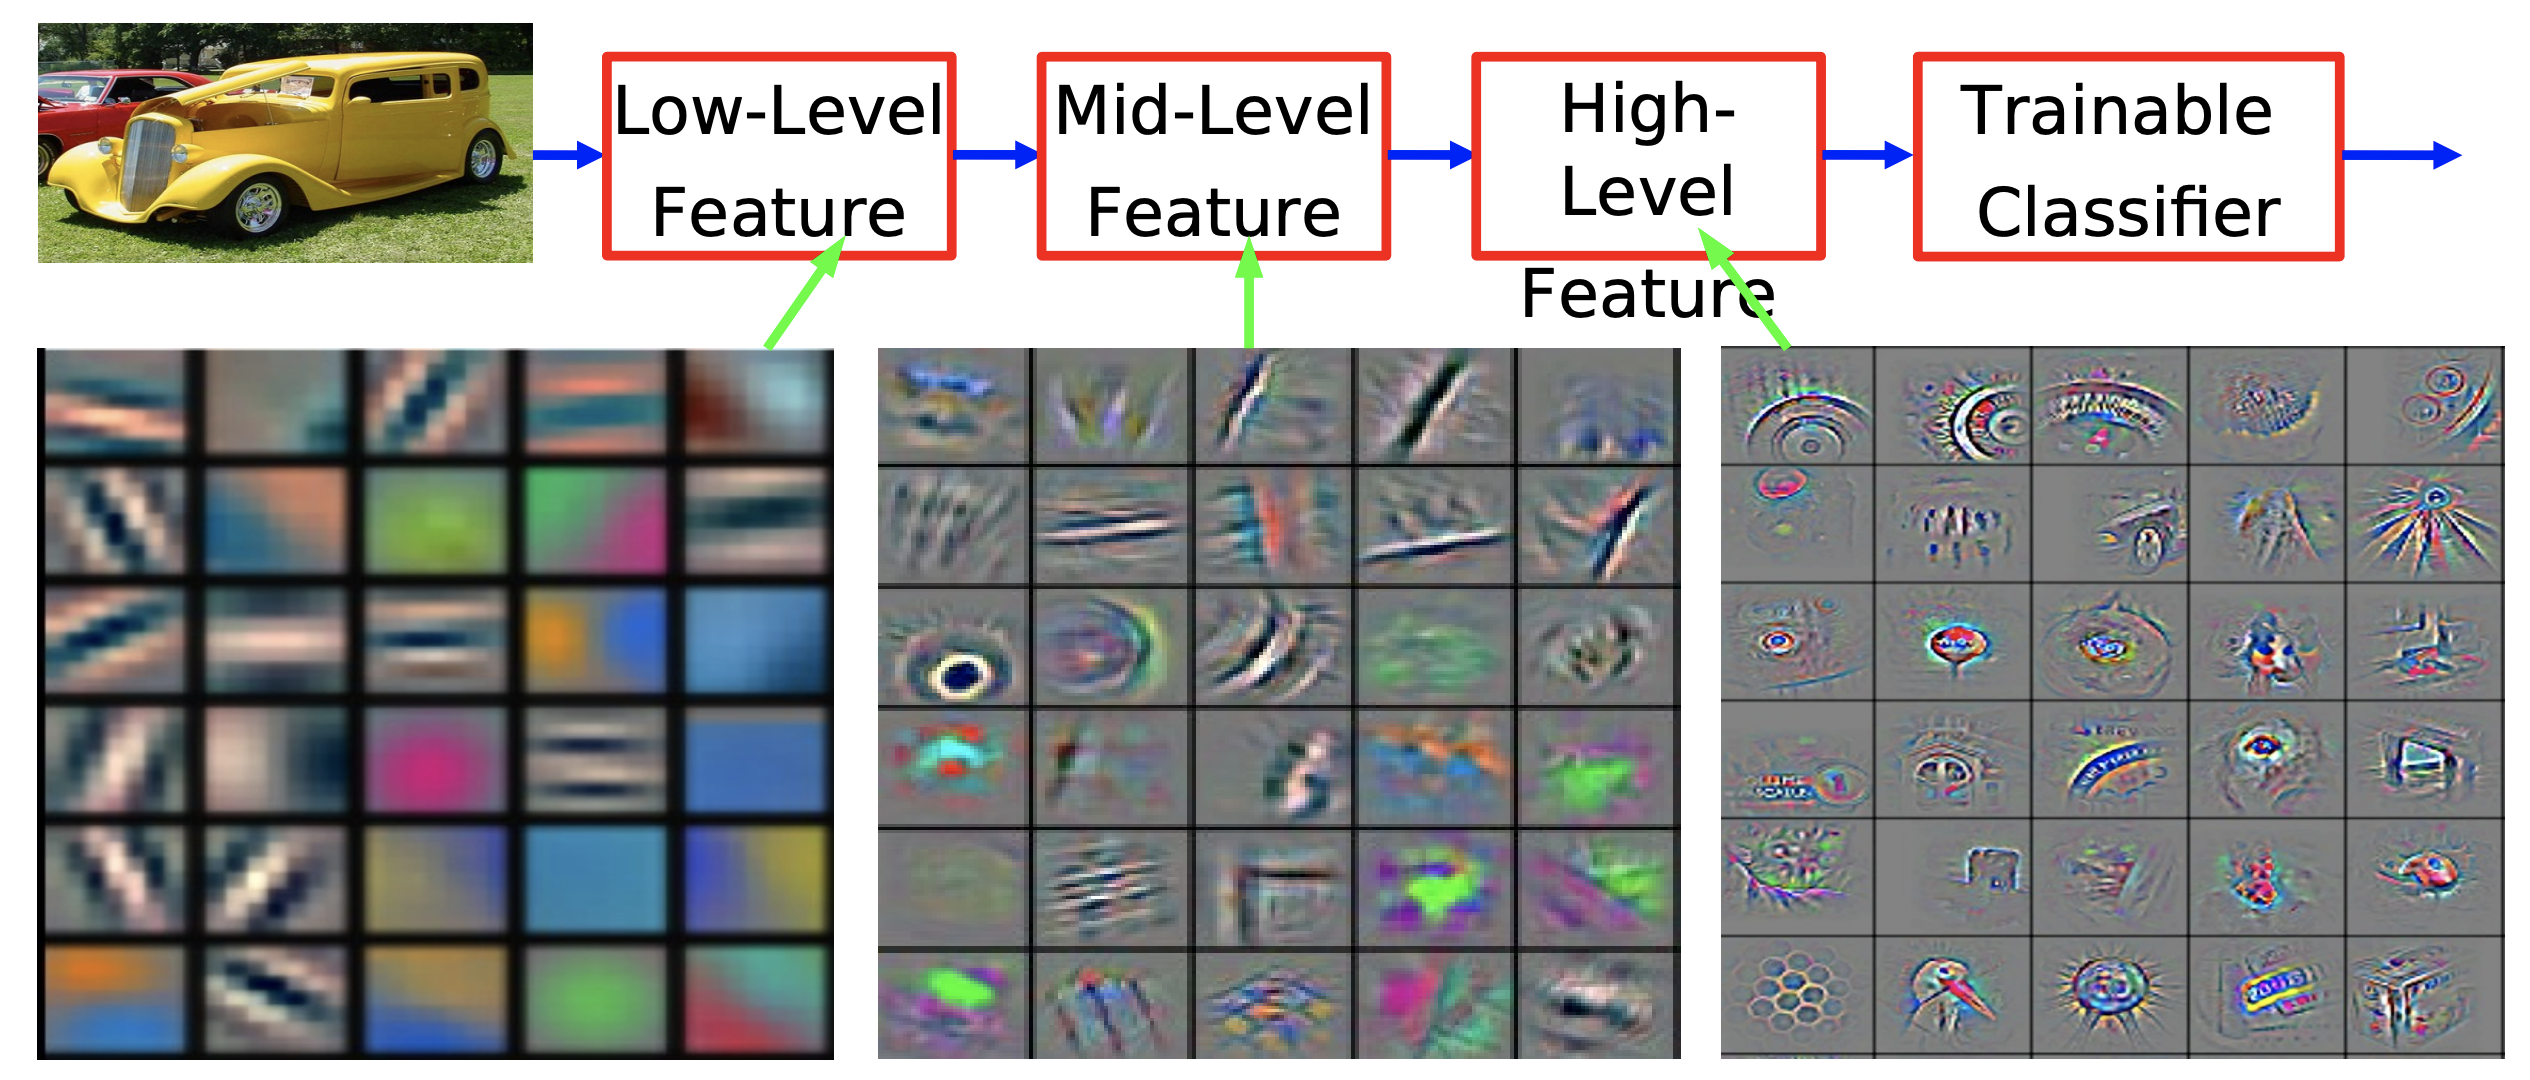
\includegraphics[width=1\textwidth]{figures/cnn_features.png}
    \caption{Feature visualization of convolutional net trained on ImageNet from \citep{zeiler2014visualizing}.
    Images to the left are features extracted in earlier layers, while images to the right are features extracted in the later layers.
    We can see earlier layer look for more simple patterns while the later layers look for more complex pattern.
    Source: \url{https://atcold.github.io/pytorch-Deep-Learning/en/week03/03-1/}}
    \label{fig:cnn_features}
\end{figure}

\subsection{Convolutional Neural Network}

Convolutional neural networks (CNNs) combine several key ideas:
\begin{enumerate}
    \item  Local Receptive Fields: Each neuron in the Neural Network receives input from neighboring neurons in a small local region of the previous layer.
    \item Weights Sharing: Neurons within the same layer share the same set of weights, as opposed to having individual weights for each neuron.
    \item Spatial Subsampling: Subsampling is performed based on region, reducing the dimension of the neural network.
\end{enumerate}

The underlying concept of CNNs is inspired by the functioning of neurons in the visual cortex of animals and humans.
This idea dates back to a paper by Hubel and Wiesel \citep{hubel1962receptive}.
Where they demonstrated that neurons in the brain of a cat are hierarchically organized and possess local receptive fields. These local receptive fields enable the detection of elementary patterns such as edges, vertices, corners, and more.

To implement this concept, weight sharing is employed.
Neurons within the same layer share an identical set of weights, leading to a reduction in the number of parameters in the neural network.
This set of weights is also called a filter/kernel.
See figure \ref{fi:weight-sharing} for an example.

\begin{figure}[!h]
    \centering
    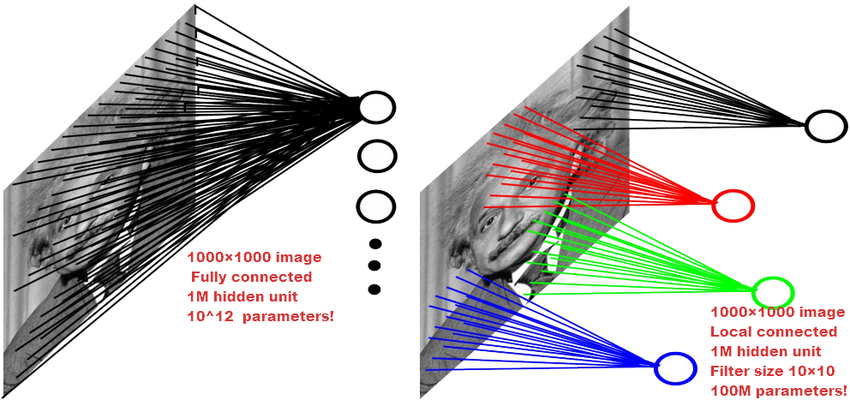
\includegraphics[width=1\textwidth]{figures/weight_Sharing_cnn.png}
    \caption{
    Comparison between a fully connected layer (left), every pixel in the image is connected to every neuron, and a convolutional layer (right), where the neurons are only locally connected.
    Source: \citep{phdthesis}
    }
    \label{fi:weight-sharing}
\end{figure}

This not only makes training and usage of the network more computationally efficient but also ensures that the network attends to the same patterns across the entire image.
These elementary patterns, identified by the kernel, are also referred to as features and are crucial building blocks for the semantic understanding of the image.

Subsequent layers in the network combine these elementary patterns to form more complex features.
See figure \ref{fig:cnn_features} for an example.
A collection of neurons within a layer is commonly referred to as a feature-/activation-map, where all neurons share the same set of weights. 
This design constraint enables the network to perform the same convolutional operation across different parts of the image.

Within a single convolutional layer, multiple filters/kernels can be employed, each focusing on different features within the image.
For instance, we could have one filter which focuses on detecting edges, while another filter identifies corners.

\subsection{Structure of CNN}

There are two essential types of layers in a CNN: convolutional layer and pooling layers.
Additional CNNs may also include fully connected layers, but they are not the core component of the CNN.
In the following sections, I want to provide an explanation of the core elements of a CNN.

\subsection{Convolutional Layer}

\begin{figure}[!h]
    \centering
    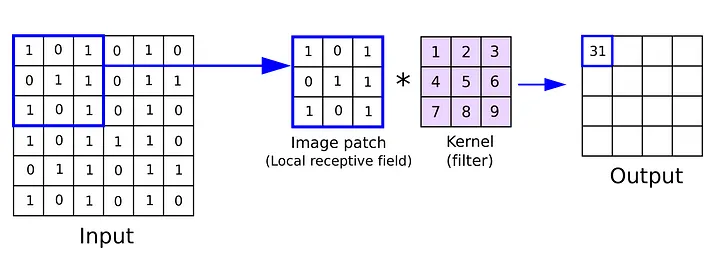
\includegraphics[width=1\textwidth]{figures/convolution_operation.png}
    \caption{Example of a convolution operation. 
    Source: \url{https://anhreynolds.com/blogs/cnn.html}}
    \label{fig:conv-op}
\end{figure}

The convolutional layer is an important building block within the CNN Architecture.
It uses weight sharing to drastically reduce the number of parameters that need to be learned by the network.

During the forward pass, the convolutional layer applies each filter/kernel by convolving it across the input, resulting in the generation of a two-dimensional activation map.

The concept of convolution arises from the \textit{convolutional operation}.
\footnote{In practice \textit{cross-correlation} is used instead, the terms \textit{convolutional operation} and \textit{cross-correlation} are often used interchangeably, although they are slightly different.}

The convolution operation $S$, with input $I$ and kernel $K$ with size, $(2N + 1)  \times (2N + 1)$\footnote{The size of the kernel doesn't need to be odd, but it is convenient, so we can suppose that as it shifts, its center is right on top of an element of image $I$.}
is defined as:
$$
S(x, y) = \sum_{j =-N}^{N}\sum_{i=-N}^{N} I(x+i, y+j)K(x,y)
$$
Essentially, the convolutional operation can be understood as 
sliding a kernel across the entire image matrix and computing the dot product between a patch from the input matrix and the kernel.

To better understand this operation, refer to figure \ref{fig:conv-op} for a graphic depiction of the operation or to \href{https://youtu.be/xjqCTp4xAtA}{\textcolor{red}{this}} for a video representation.

Two important hyperparameters are associated with the convolution operation:
\begin{itemize}
    \item The first is stride, which determines the number of pixels the kernel slides by during each operation. For example, a stride of 1 means that the sliding window moves 1 pixel at a time.
    \item The second hyperparameter is the kernel size, which determines the dimensions of the kernel sliding over the input image. For instance, a kernel size of 4×4 indicates that we have a kernel matrix of size 4×4 that slides over the input matrix.
\end{itemize}
The kernel size can also be understood as the size of the local receptive field of the neurons.
 
\subsection{Subsampling}

\begin{figure}[!h]
    \centering
    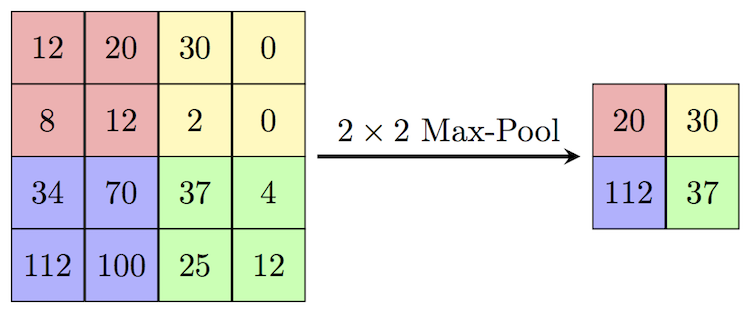
\includegraphics[width=1\textwidth]{figures/MaxpoolSample2.png}
    \caption{Demonstration of the max-pooling operation with stride 2 and filter
size 2x2. We go over each image patch and take the highest value. Source:
\url{https://computersciencewiki.org/index.php/File:MaxpoolSample2.png}}
    \label{fig:subsampling}
\end{figure}

Training an infinitely large neural network is not feasible due to the increasing computational costs associated with both training and inference.
Therefore, it is essential to ensure that a network is not unnecessarily larger than necessary.
One way to achieve this is by reducing the dimensions of the network layers, where the dimension means the number of neurons in a layer.

To accomplish dimension reduction, subsampling techniques can be employed. Two popular subsampling methods are average pooling and max pooling.

In average pooling, similar to convolution layers, we slide over our image matrix and take the average of a neighborhood region in the image and map it to a single neuron in the next layer.
On the other hand, in max pooling, the highest value within a neighborhood region is selected and mapped to a neuron in the subsequent layer.
See figure \ref{fig:subsampling} for an example of max pooling.

The max-pooling operation can be seen as propagating only the most significant signal that excites a neuron the most while discarding the rest. This approach bears some resemblance to the way the brain processes information.
What type of pooling layer is better is highly dependent on the task \citep{app12178643}.

\begin{wrapfigure}{r}{0.3\linewidth}
    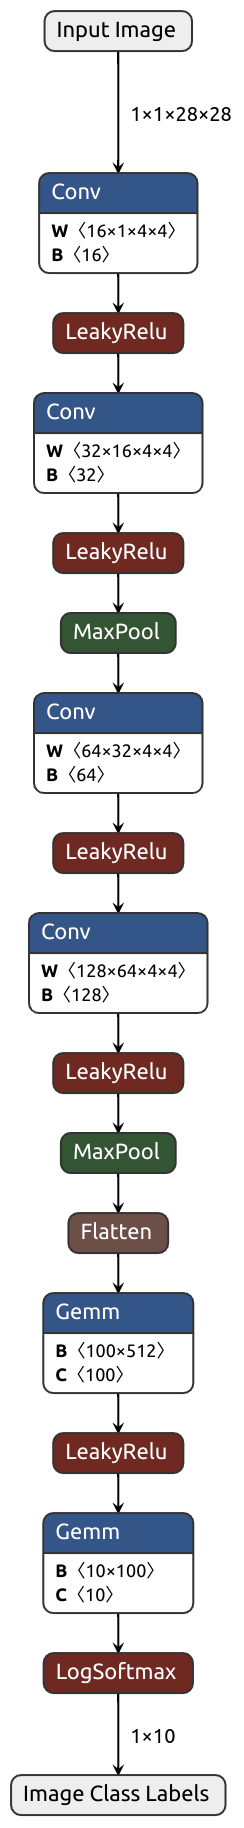
\includegraphics[width=0.6\linewidth]{figures/CNN_Architetcure.png}
    \caption{The architecture of the Baseline CNN-Model.}
    \label{fig:architecture}
    \vspace{-100pt} 
\end{wrapfigure}

Both of these approaches aid in reducing the dimension of the network.

\section{Self-Trained CNN}

In order to demonstrate the effectiveness of a CNN, I conducted an experiment where I trained a CNN from scratch to recognize black-and-white digits from images.

The code I used to train and evaluate the models is available at \url{https://github.com/LuposX/SeminareCNN/tree/main}.

\subsection{Dataset}


I trained my CNN using the MNIST dataset \citep{CNNLeCunDocumentRecog}, the MNIST dataset is a collection of 70,000 hand-drawn digits. 
These digits are gray-scaled images and have been normalized to fit within a 28×28 pixel bounding box.

I choose this dataset due to its popularity within the machine learning community and its low computational requirements.

Moreover, the dataset was commonly used for evaluating the performance of CNNs.
The MNIST  dataset is divided into 60,000 training images and 10,000 testing images.
To prepare the image for training, I normalize them to ensure that the input data has a mean of 0 and a standard deviation of 1, which can improve the stability of the learning process. \citep{589532}.

\subsection{Architecture}

The CNN architecture, as illustrated in Figure \ref{fig:architecture}, consists of 6 layers with learnable weights. The initial 4 layers are convolutional, while the subsequent 2 layers are fully connected.

The first convolutional layer takes a 28×28×1 \footnote{This refers to (Image Width $\times$ Image Height $\times$ Number of Color Channels).} image as input and applies 16 filters to extract relevant features.
Subsequent convolutional layers have the following number of filters: 32, 64, and 128.

To reduce the spatial dimension of the feature maps, a max pooling layer is applied every two convolutional layers.
This layer uses a kernel size of 2x2 with a stride of 2, effectively halving the spatial dimension of the image.

Transitioning to the fully connected layers, the network contains 5776, 200, and 10 neurons, respectively. As activation-function, Leaky ReLU is applied to all layers except the last one. Leaky Relu has the advantage over ReLu that it leads to a slightly more stable learning process \footnote{It solves the problem of dead-ReLus.} \citep{Maas2013RectifierNI}.
Formally, the Leaky ReLu function is defined as: 
$$
f(x) =
\begin{cases}
x \qquad \ \text{if } x >0, \\ 
\alpha \cdot x \quad \text{otherwise.}
\end{cases}
$$
where $\alpha = 0.2$ this value was determined to be effective based on findings from the paper \citep{xu2015Reluempirical}.

The final layer's output is passed through a 10-way log-softmax function, generating a probability distribution across 10 class labels. Formally, the log-softmax function is defined as: 
$$
\text{LogSoftmax}(x_i) = log(\frac{\text{exp}(x_i)}{\sum_{j \in \{0, 1, ..., 9\}}\text{exp}(x_j)})
$$
Applying log-softmax in combination with \textit{negative log-likelihood loss} has several advantages, its primary benefit being its numerical properties that contribute to faster training time.

We can interpret the output of the neurons as the model's confidence in each class label.
A high output value associated with a specific label indicated that the model thinks that label is more probable to be the correct output.

\subsection{Trainings-Details}

The model was trained using the backpropagation algorithm and the \textit{negative log likelihood} \footnote{Is defined as $L(X, Y) := -log(p(Y | X))$} loss function, which is commonly used for multi-class classification tasks.

For efficient training, Google Colab was used, taking advantage of the free dedicated GPU to  accelerate the training process.

The CNN was trained for 5 epochs using a batch size of 1024.
The total training time was approximately 5 minutes.

As training optimizer, Adam was used with a learning rate of 0.001. Adam is a state-of-the-art optimizer known for its ability to adaptively adjust learning rates during training and the use of momentum \citep{kingma2014adam}.

\subsection{Results \& Ablation Study} \label{resultsAbalation}

To assess the robustness of Convolutional Neural Network(CNN) compared to fully connected neural networks(FCNN), I experimented with both architectures.
In addition to the CNN-Model, I trained an additional FCNN once on the original dataset and once on a modified dataset, on which I applied various transformations.
The transformation applied to the dataset were as follows:
\begin{itemize}
    \item  Adding Random Noise: I generated random tensors of the same size as the input images. These tensors were sampled from a Gaussian Distribution $N$  \footnote{$N \sim \mathcal{N}(0.6, 0)$, the standard deviation in this case can be interpreted as the intensivity of the noise.}, I added these sampled tensors to the corresponding images.
    \item Random Image Cropping: All images in the dataset were randomly cropped, resulting in images that were no longer centered.
\end{itemize}
A sample from the modified dataset can be seen in figure \ref{fig:modified-dataset}.

After performing these transformations, I trained a new CNN model (referred to as \textit{CNN\_Noise\_RandomCrop}) with the same architecture as the original model, using the transformed dataset.
Additionally, I trained an FCNN of equivalent size \footnote{Size refers here to the parameter count, for more information about the architecture of the FCNN model check the projects GitHub page.} as the CNN model.
The FCNN was trained twice, once on the original dataset (referred to as \textit{FC\_NN}) and once on the transformed dataset (referred to as \textit{FC\_NN\_Noise\_RandomCrop}).

As depicted in figure \ref{fig:results} the CNN trained on the original dataset achieved a performance of approximately 99\%.
However, when I trained on the transformed dataset, the CNN's accuracy decreased to 92\%.
On the other hand, the FCNN achieved an accuracy of 95\% when trained on the original dataset.
When trained on the transformed dataset, the FCNN's accuracy dropped significantly to 75\%.

These outcomes demonstrate the robustness of CNNs, as they exhibit greater resilience to image transformations, as explained in Section \ref{CNN}.

\begin{figure}%{r}{0.3\linewidth}
    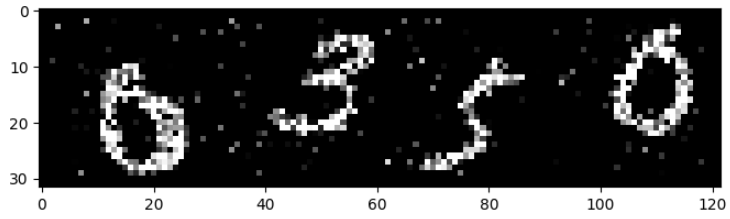
\includegraphics[width=1\linewidth]{figures/sample_modified_dataset.png}
    \caption{Sample Data from the modified MNIST dataset.}
    \label{fig:modified-dataset}
    %\vspace{-25pt}
\end{figure}

\begin{figure}[h]
    \begin{subfigure}[b]{0.5\textwidth}
        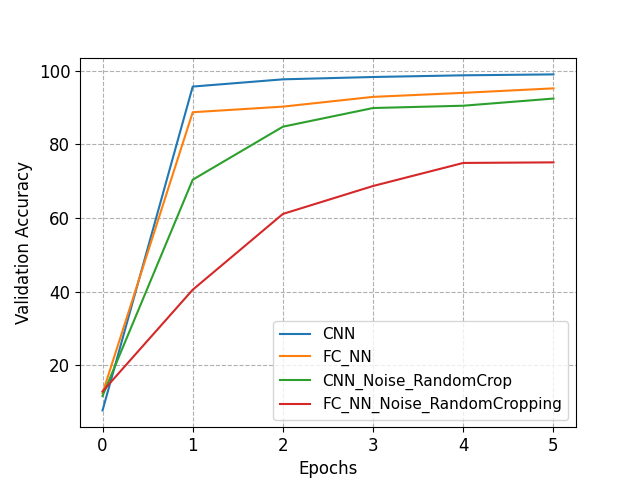
\includegraphics[width=\textwidth]{figures/val_acc_result_data.png}
        \caption{The Validation Accuracy}
    \end{subfigure}
     \begin{subfigure}[b]{0.5\textwidth}
        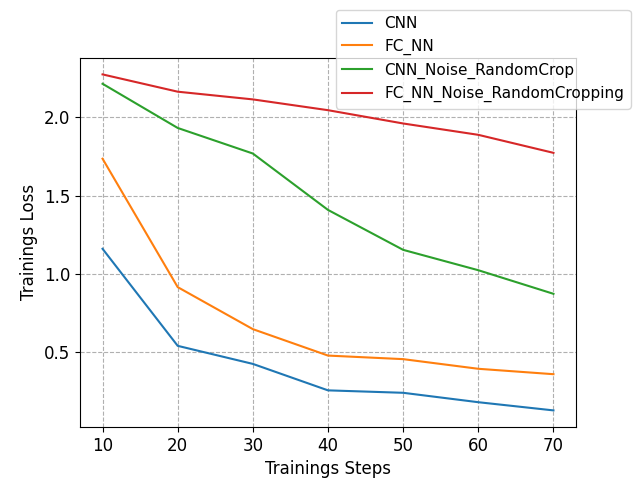
\includegraphics[width=\textwidth]{figures/train_loss_accumulated_result_data.png}
        \caption{The trainings Loss}
    \end{subfigure}
    \caption{Following abbreviations apply CNN = Convolutional Neural Network, FC\_NN = Fully Connected Neural Network, Noise = Random Noise was added do the training's data, RandomCrop = the training data was randomly cropped.}
    \label{fig:results}
\end{figure}

\section{Conclusion \& Discussion}

This proseminar provides an overview of CNNs, including their definition and functionality.
Additionally, a practical demonstration was conducted aimed to show the capabilities of CNNs and illustrate how a CNN architecture might look like.
This serves as an example to showcase the effectiveness of CNNs and provide insight into their architectural structure.

It would have been interesting to investigate the possibility to make the FCNN more competitive with the CNN through the use of additional techniques.

\section{Acknowledgment}

I would like to thank Yuri Koide for giving me pointers while I was working on the slides to present the topic of this proseminar.

